\section{Class M1: every forward run short}\label{sec:short-runs}

A period of class \cls{M1} is mixed, every maximal run of reverse switches has length two and
every maximal run of forward switches has length one (\cref{def:classes}). Its cyclic sign word is
therefore $(--+)^m$: every reverse run is a pair of reverse switches around a centre piece, and
consecutive pairs are separated by single forward switches. This section proves the following
theorem.

\begin{theorem}\label{thm:class-M1}
  No competitive normal vertex period belongs to class \cls{M1}.
\end{theorem}

The theorem uses neither the compact domain nor a lower bound on the number of pieces. Its proof
compares two ways of counting how far the switch vectors $y_k$ of \cref{def:normal-multiplier}
turn in one period, measured in the positive definite form $S$. At a turn the switch vector only
changes sign, so all the turning happens at the $m$ centres. A whole-period winding identity fixes
the total turning at exactly $(m+1)\pi/3$, because the frame of a competitive period turns by
exactly $\pi/3$. A local estimate at each centre, which combines the stationarity identity, the
Gram identity and the competitive cap on the Casimir $\gamma^2$, shows that each centre turns the
switch vectors by more than $2\pi/5$. The average $(m+1)\pi/(3m)$ is at most $2\pi/5$ as soon as
$m\ge5$, and the word condition leaves $m=2$ as the only other case. With two centres the
recurrence of the switch vectors closes up only in a rigid configuration whose cost can be computed
exactly, and it exceeds $\Aoct$.

\subsection{The sign word}

\begin{lemma}\label{lem:m1-pattern}
  Let a vertex representation with $N$ pieces belong to class \cls{M1}. Then $N=3m$ for an integer
  $m\ge1$ with $m\equiv2\pmod 3$, and there is $k_0\in\Z$ such that for every $j\in\Z$ the
  switches $k_0+3j$ and $k_0+3j+1$ are reverse and the switch $k_0+3j+2$ is forward.
\end{lemma}

\begin{proof}
  A mixed representation has a forward switch followed by a reverse one: otherwise every switch
  after the first forward one would be forward, which the periodicity $\varepsilon_{k+N}=\varepsilon_k$
  of the signs forbids. Start at such a pair. The reverse run that begins there has length two,
  and the forward run that follows it has length one, so the signs continue as
  $-,-,+,-,-,+,\dots$ with period three. Hence $N=3m$ and the word is $(--+)^m$. The signs of one
  period add up to $m-2m=-m$, and \cref{lem:sign-sum} gives $-m\equiv1\pmod3$.
\end{proof}

We fix $k_0$ and $m$ as in the lemma and call the piece $c_j=k_0+3j+1$, which lies between the two
reverse switches of the $j$-th run, the $j$-th \emph{centre}. The pieces $c_j+1$ and $c_j+2$ are
turns: one of their two switches is forward and the other reverse. At a turn the outgoing switch
vector is the negative of the incoming one, so the three switch vectors that follow the centre
$c_j$ are $z_j$, $-z_j$, $z_j$ with $z_j=y_{c_j}$. Between two consecutive centres the switch
vectors therefore do not turn, and the whole turning of the sequence $(y_k)$ is concentrated at
the centres.

\subsection{The data at a centre}

Fix a centre $c$, with active margin $a=a_c$ and neighbouring active margins $p=a_{c-1}$ and
$n=a_{c+1}$. In this section we write
\begin{equation}\label{eq:m1-variables}
  \begin{gathered}
    r=\frac a{a+p},\qquad t=\frac a{a+n},\qquad \rho=\frac{a^2}{a^2+4},\\
    u=8d_{c-1},\qquad v=8d_c,\qquad E=16e_c,\qquad U(s)=1-s+s^2.
  \end{gathered}
\end{equation}
Here $d_{c-1}$ and $d_c$ are the switch norms of the two reverse switches at the ends of the
centre and $e_c$ is the cross pairing on the centre. The letter $\rho$ is local to this section.

\begin{lemma}\label{lem:m1-centre-data}
  Let $P$ be a normal vertex period with the sign word of \cref{lem:m1-pattern}, and let $\gamma^2$
  be its Casimir. At every centre the numbers \eqref{eq:m1-variables} satisfy
  \begin{enumerate}[label=\textup{(\roman*)}]
    \item $0<r<\tfrac12$, $0<t<\tfrac12$ and $0<\rho<rt$;
    \item $\tfrac34\le u\le U(r)$ and $\tfrac34\le v\le U(t)$;
    \item the stationarity identity
    \begin{equation}\label{eq:m1-stat}
      E=1+r+t-\rho+\log\frac{\rho}{rt}-\frac{1-u}r-\frac{1-v}t;
    \end{equation}
    \item the Gram identity $16(1-\rho)^2\gamma^2=4uv-E^2$.
  \end{enumerate}
\end{lemma}

\begin{proof}
  (i) The centre is the middle piece of a reverse run of length two, so its active margin is
  strictly smaller than both neighbouring ones (\cref{prop:run-structure}). This gives
  $r,t<1/2$. The factor of the centre is $q_c=(a^2+4)/((a+p)(a+n))$, and $q_c>1$ is the
  inequality $(a+p)(a+n)<a^2+4$, which is $\rho<rt$.

  (ii) Both neighbours of the centre are turns. The switch norms at the two ends of a turn are
  equal and at least $3/32$ (\cref{lem:switch-norms}); this gives $u,v\ge 3/4$. Both switches of
  the centre are reverse, so $d_{c-1}\le j_{c-1}/2$ and $d_c\le j_c/2$ by \cref{lem:switch-norms},
  and $4j_{c-1}=(a^2+ap+p^2)/(a+p)^2=U(r)$, and likewise $4j_c=U(t)$.

  (iii) is the stationarity identity of \cref{lem:stationarity} with both incident signs equal to
  $-1$, written in the variables \eqref{eq:m1-variables}.

  (iv) is the Gram identity $d_{c-1}d_c-e_c^2=\gamma^2/(a^2+4)^2$ at a centre (\cref{lem:gram}),
  multiplied by $256$, since $1-\rho=4/(a^2+4)$.
\end{proof}

Since the period is mixed, $\gamma^2>0$ (\cref{prop:ellipticity}), and the switch norms are
positive. The form $S$, whose determinant is $\gamma^2$, is then positive definite, and the number
\[
  \cos\varphi_c=\frac{e_c}{\sqrt{d_{c-1}d_c}}=\frac{E}{2\sqrt{uv}}
\]
is the cosine of the angle $\varphi_c\in(0,\pi)$ between $y_{c-1}$ and $y_c$ in the inner product
$S$; by (iv) its absolute value is less than one. The determinant $\det(y_{c-1},y_c)=-1/(a^2+4)$
is negative at every centre, so all the centres turn the switch vectors in the same sense. We call
$\varphi_c$ the \emph{centre angle}.

\subsection{The angle gap}

A centre with a large angle cosine needs a large pairing $E$. The stationarity identity
\eqref{eq:m1-stat} allows a large $E$ only when $\log(\rho/(rt))$ is not too negative, that is,
when the centre margin is not too small compared with its neighbours. A large centre margin makes
the factor $16(1-\rho)^2$ in the Gram identity (iv) small, and then (iv) forces the Casimir
$\gamma^2$ up, against the competitive cap of \cref{cor:casimir-cap}. The next proposition makes
the conflict quantitative.

\begin{proposition}\label{prop:m1-angle-gap}
  Let $\gamma^2,r,t,\rho,u,v,E$ be real numbers satisfying \textup{(i)--(iv)} of
  \cref{lem:m1-centre-data}, and suppose that $\gamma^2\le 97969/529200$. Then
  $E<\frac35\sqrt{uv}$; that is, $\cos\varphi<3/10$ for $\cos\varphi=E/(2\sqrt{uv})$.
\end{proposition}

The proof, in \cref{app:short-run-estimates}, reduces the seven variables to two in three steps.
Write $E=(1-\rho+\log\rho)+\Psi(r,u)+\Psi(t,v)$ with $\Psi(r,u)=r-\log r-(1-u)/r$, and let
$\omega(x)=-x-\log(1-x)=\sum_{n\ge2}x^n/n$ for $0\le x<1$.
\begin{enumerate}[label=(\alph*)]
  \item One reverse switch at a time: for $s=\sqrt{4u-3}$ one has $u=U((1-s)/2)$, $2r\le 1-s$, and
  $\Psi(r,u)\le\omega(s)+\log2$, with equality when $r=(1-s)/2$, that is, when the switch bound
  $u\le U(r)$ is attained.
  \item The two switches together: define $S\ge0$ by $S^2=s^2+s'^2+s^2s'^2/3$, where
  $s'=\sqrt{4v-3}$. Then $uv=3(3+S^2)/16$, and $\omega(s)+\omega(s')\le\omega(S)$ because
  $\omega$ is superadditive in $x^2$.
  \item The centre: $z=4\rho/(1-S)$ lies in $(0,1]$, $\rho=(1-S)z/4$, and
  $E\le(1-S)(1-z/4)+\log z$.
\end{enumerate}
If $\cos\varphi\ge3/10$, then $E^2\ge\frac{9}{25}uv$, and the two-variable inequality of
\cref{lem:m1-core} gives $16K_*(1-\rho)^2<4uv-E^2$ for the cap $K_*=97969/529200$, which
contradicts (iv). \Cref{fig:short-runs-gap} shows the region of $(S,z)$ that survives the
reductions and the least Casimir compatible with it.

\begin{figure}[htbp]
  \centering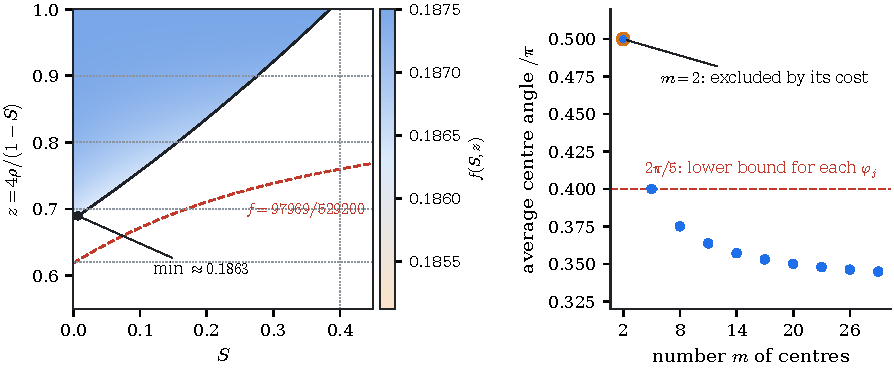
\includegraphics[width=\textwidth]{figures/fig-short-runs-gap.pdf}
  \caption{Left: the reduced variables of the angle gap. The shaded region is the set of
  $(S,z)$ with $(1-S)(1-z/4)+\log z\ge\frac35\sqrt{3(3+S^2)/16}$, where a centre with
  $\cos\varphi\ge3/10$ must lie; on it the colour is the least Casimir
  $f(S,z)=(4Q-E_{\max}^2)/(16(1-\rho)^2)$ allowed by the Gram identity, with
  $Q=3(3+S^2)/16$, $E_{\max}=(1-S)(1-z/4)+\log z$ and $\rho=(1-S)z/4$. Its minimum is about
  $0.1863$, attained near $S=0$, and the level set $f=97969/529200\approx0.18513$ of the cap
  (dashed) stays outside the region. The dotted lines are $S=2/5$, $z=31/50$ and the ends of the
  four tangent-line intervals of \cref{lem:m1-core}. Right: the average centre angle
  $(m+1)\pi/(3m)$ forced by the winding identity, for $m\equiv2\pmod3$, against the lower bound
  $2\pi/5$ for every centre angle. The two meet at $m=5$; only $m=2$ lies above the
  line.}\label{fig:short-runs-gap}
\end{figure}

\begin{corollary}\label{cor:m1-angle}
  At every centre of a competitive normal vertex period of class \cls{M1}, $\varphi_c>2\pi/5$.
\end{corollary}

\begin{proof}
  The Casimir and the first switch norm are positive, so the competitive cap
  $\gamma^2\le97969/529200$ of \cref{cor:casimir-cap} applies. By \cref{lem:m1-centre-data} and
  \cref{prop:m1-angle-gap}, $\cos\varphi_c<3/10$. Since $\cos(2\pi/5)=(\sqrt5-1)/4>3/10$, which
  is $\sqrt5>11/5$, and the arccosine decreases, $\varphi_c>2\pi/5$.
\end{proof}

\begin{remark}\label{rem:m1-route-gap}
  Another argument for \cref{prop:m1-angle-gap} is given in \cite{Notes}
  (\texttt{MIXED\_GLOBAL\_SHORT\_RUN\_ANGLE\_EXCLUSION}). At a fixed cosine $c$ it solves the
  stationarity identity for $\rho$ and follows a path along which the Casimir does not increase,
  to the symmetric configuration $r=t=1/2$, $u=v=3/4$; there $1-\rho_c+\log(4\rho_c)=3c/2$, and a
  rational separation at $\rho=17/100$ beats the cap. Both arguments meet at the same extremal
  configuration: $S=0$ is $u=v=3/4$, and on $S=0$ the boundary of the region in
  \cref{fig:short-runs-gap} is the equation for $\rho_c$, with $c=3/10$ and $z=4\rho_c$.
\end{remark}

\subsection{The winding identity}

\begin{proposition}\label{prop:m1-winding}
  Let $P$ be a competitive normal vertex period with the sign word of \cref{lem:m1-pattern}, $N=3m$,
  and positive Casimir. Then
  \[
    \sum_{j=0}^{m-1}\varphi_{c_j}=\frac{(m+1)\pi}3,\qquad
    \varphi_c=\arccos\frac{E_c}{2\sqrt{u_cv_c}},
  \]
  where $E_c,u_c,v_c$ are the numbers \eqref{eq:m1-variables} at the centre $c$.
\end{proposition}

The identity says that the switch vectors, which turn only at the centres, turn in total by the
angle that the frame of the period prescribes. The proof expresses the switch vectors through the
physical frame and follows a continuous angle along the period.

\runin{Switch vectors in the physical frame.} Let $V(t)=g(t)X(t)$ be the tangent frame. The
switch vector at the switch $n$ is, up to a sign and a positive factor, $KV(\tau_n)b$, where
$K=R^{i_0}C(-X(0))$ is a fixed matrix with $\det K=-2\sqrt3$, $C$ is the triangular change of
coordinates, and $b$ is one of two base vectors $b_{\mathrm{in}}(i)$ and
$b_{\mathrm{out}}(i)=Rb_{\mathrm{in}}(i)$ that depend only on the label $i$ of the piece. Factor
$S=Q^{\mathsf T}Q$ with $\det Q<0$, so that angles for $S$ become Euclidean angles after $Q$.

\runin{A continuous angle.} The polar number $z(g)=(g_{00}+g_{11})/2+i(g_{10}-g_{01})/2$ of a
matrix of determinant one has modulus at least one, and for every vector $w\ne0$ the quotient
$gw/(z(g)w)$ lies in the right half-plane, since
$\operatorname{Re}\bigl(gw\cdot\overline{z(g)w}\bigr)=(\abs{gw}^2+\abs{w}^2)/2$. Let $\Phi(t)$ be a
continuous angle of $z(g(t))$. For $w\ne0$ let $\kappa_t(w)$ be the angle from $w$ to
$QKg(t)X(t)w$ obtained by adding $\Phi(t)$ to principal arguments that never leave the slit
plane; it depends continuously on $t$.

\runin{Three facts.} At a centre $c$ the centre angle is
$\varphi_c=\pi/3+\kappa_{\tau_c}(b_{\mathrm{out}})-\kappa_{\tau_c}(b_{\mathrm{in}})$. Along a piece
the base vector that is being followed is an eigenvector of the tangent factor of the piece, so
$g(t)X(t)b$ keeps its direction and $\kappa_t(b)$ is constant; between consecutive centres the
outgoing base vector of one is, up to sign, the incoming base vector of the next. Across the
seam, $\kappa_T(w)=\kappa_0(Rw)+\pi/3$, because $g(0)=I$, $g(T)=R$ and $\Phi(T)-\Phi(0)=\pi/3$.

\runin{The frame turns by exactly $\pi/3$.} The endpoint conditions fix $\Phi(T)-\Phi(0)$ only
modulo $2\pi$. For a competitive period the cost is at most $\Aoct<\pi$, and the winding theorem
behind the reverse comparison (\cref{prop:reverse-comparison}) shows that the reflected first row
$(g_{00},-g_{01})$ of the frame turns by exactly $\pi/3$. The real part of the product of that row
with the conjugate of $z(g)$ is $(g_{00}^2+g_{01}^2+1)/2>0$, so the two angles stay within $\pi/2$
of each other, and $\Phi(T)-\Phi(0)=\pi/3$.

\runin{Telescoping.} The centre angles are periodic in $j$ with period $m$, so we may take the $m$
centres of one period in a window that starts at the seam. Summing the centre formula over them,
the term $\kappa(b_{\mathrm{out}})$ of each centre cancels the term $\kappa(b_{\mathrm{in}})$ of
the next, and the last link crosses the seam, where it gains $\pi/3$. What remains is
$m\cdot\pi/3+\pi/3$.

\begin{remark}\label{rem:m1-route-winding}
  The identity can also be derived from the universal cover of $\SLtwo$ (\cite{Notes},
  \texttt{MIXED\_GLOBAL\_PROJECTIVE\_WINDING}). The tangent frame $X(0)^{-1}g(t)X(t)$ has the
  relative homotopy class of the canonical path from $I$ to $R$; the cyclic product of the factors
  $T_0(q_k)R^{-\varepsilon_k}$ then lifts to the central element $\widetilde R^{-3\ell}$, where
  $\sum\varepsilon_k=3\ell+1$. Identify the vectors at the turns, and change the sign of the
  representative across every centre, so that every centre contributes $\pi-\varphi_c$. The total
  is $n\pi$ with $n=(N-m-1)/3=(2m-1)/3$, which is the same identity:
  $m\pi-\sum_j\varphi_{c_j}=(2m-1)\pi/3$.
\end{remark}

\subsection{Five or more centres}

\begin{proof}[Proof of \cref{thm:class-M1} for $m\ge5$]
  By \cref{cor:m1-angle} every centre angle exceeds $2\pi/5$, so the sum in
  \cref{prop:m1-winding} exceeds $2m\pi/5$. For $m\ge5$, $2m/5\ge(m+1)/3$, which contradicts
  \cref{prop:m1-winding}. Since $m\equiv2\pmod3$, the only other case is $m=2$.
\end{proof}

\subsection{Two centres}

For $m=2$ the average centre angle is $\pi/2>2\pi/5$, and the angle count gives nothing. The
argument uses instead the recurrence of the switch vectors and the cost identity. For the centre
$c_j$ put $K_j=a_{c_j}^2+4$, write $b_j=a_{c_j+1}$ and $b'_j=a_{c_j+2}$ for the active margins of
the two turns that follow it, and
\[
  D_j=(a_{c_j}+b_j)^2+(b'_j+a_{c_{j+1}})^2-(b_j+b'_j)^2=s_{c_j}^2+s_{c_j+2}^2-s_{c_j+1}^2 .
\]

\begin{lemma}\label{lem:m1-recurrence}
  In a normal vertex period with the sign word of \cref{lem:m1-pattern}, the vectors $z_j=y_{c_j}$
  satisfy
  \[
    K_{j+1}z_{j+1}=-K_jz_{j-1}+D_jz_j,\qquad \det(z_{j-1},z_j)=-1/K_j,
  \]
  and the cyclic product of the period is $\pm I$, so that $z_{j+m}=\pm z_j$ with one sign for all
  $j$.
\end{lemma}

\begin{proof}
  Work in triangular coordinates and in the frame of the centre $c=c_j$, that is, multiply all
  vectors by the inverse of the prefix product up to $c$. Put $A_\pm(q)=T_0(q)R^{\mp1}$, so that
  \[
    A_+(q)=\begin{pmatrix}q&-q\\ 1/q&0\end{pmatrix},\qquad
    A_-(q)=\begin{pmatrix}0&q\\ -1/q&1/q\end{pmatrix},
  \]
  and write $K=K_j$ and $s_k=a_k+a_{k+1}$. The factors of the centre and of the two turns after it
  are $K/(s_{c-1}s_c)$, $s_{c+1}/s_c$ and $s_{c+1}/s_{c+2}$. In this frame
  $z_{j-1}=-(1/s_{c-1},0)^{\mathsf T}$ and $z_j=(0,s_{c-1}/K)^{\mathsf T}$, which gives the
  determinant, and
  \begin{align*}
    K_{j+1}z_{j+1}
    &=s_{c+2}\,A_-\Bigl(\frac K{s_{c-1}s_c}\Bigr)A_+\Bigl(\frac{s_{c+1}}{s_c}\Bigr)
      A_-\Bigl(\frac{s_{c+1}}{s_{c+2}}\Bigr)\begin{pmatrix}0\\1\end{pmatrix}
    =\begin{pmatrix}K/s_{c-1}\\ (s_{c-1}/K)\,D_j\end{pmatrix}\\
    &=-Kz_{j-1}+D_jz_j .
  \end{align*}
  Multiplying back by the prefix product preserves the recurrence and the determinant. The
  cyclic product of the period is $\pm I$ by the tangent closure (\cref{lem:tangent-closure}).
\end{proof}

\begin{lemma}\label{lem:m1-euler}
  For every normal vertex period,
  \[
    \frac{2\cost}{\sqrt{12}}
    =8\sum_{k=0}^{N-1}(\varepsilon_{k-1}+\varepsilon_k)e_k
      -2\sum_{k=0}^{N-1}\frac{\varepsilon_{k-1}+\varepsilon_k}{a_k^2+4}.
  \]
\end{lemma}

\begin{proof}
  Multiply the stationarity identity of \cref{lem:stationarity} at the piece $k$ by $a_k$ and sum
  over a period. The switch norms and the cross pairings are formed from one weight $w_k$ per piece,
  $d_k=(w_k+w_{k+1})/(2s_k^2)$ and $e_k=w_k/(2(a_k^2+4))$. Regrouped by switches, the left-hand
  sides add up to $\sum_k(\varepsilon_{k-1}+\varepsilon_k)w_k\bigl(1-a_k^2/(a_k^2+4)\bigr)
  =8\sum_k(\varepsilon_{k-1}+\varepsilon_k)e_k$. On the right-hand side, the one-arc cost formula
  of \cref{lem:one-arc}, with the factors written in the active margins, gives
  $8\cost/\sqrt{12}=\sum_k\varepsilon_kG(a_k,a_{k+1})$ for the signed action
  \[
    G(a,b)=3ab-4-(a^2+b^2)\log(a+b)+\tfrac12a^2\log(a^2+4)+\tfrac12b^2\log(b^2+4),
  \]
  and the stationarity identity involves the partial derivatives of $G$. The Euler-type identity
  $aG_a(a,b)+bG_b(a,b)=2G(a,b)+16/(a^2+4)+16/(b^2+4)$ turns the sum of the right-hand sides into
  $2\cost/\sqrt{12}+2\sum_k(\varepsilon_{k-1}+\varepsilon_k)/(a_k^2+4)$.
\end{proof}

In the word $(--+)^m$, $\varepsilon_{k-1}+\varepsilon_k$ is $-2$ at a centre and $0$ at a turn,
so the lemma reads $\cost/\sqrt{12}=2\sum_j1/K_j-8\sum_je_{c_j}$.

\begin{proposition}\label{prop:m1-two-centre}
  A competitive normal vertex period with $N=6$ does not have the sign word $(--+)^2$.
\end{proposition}

\begin{proof}
  The two recurrences of \cref{lem:m1-recurrence} read $K_1z_1=-K_0z_{-1}+D_0z_0$ and
  $K_0z_2=-K_1z_0+D_1z_1$, with $z_{-1}=\pm z_1$ and $z_2=\pm z_0$, and $z_0,z_1$ are independent.
  The sign $+$ would give $(K_0+K_1)z_1=D_0z_0$, which is impossible. So $z_{-1}=-z_1$, and the
  recurrences give $K_0=K_1$ and $D_0=D_1=0$. Hence both centres have the same active margin $a$,
  $K=a^2+4$, and $e_{c_0}=z_{-1}^{\mathsf T}Sz_0=-e_{c_1}$. \Cref{lem:m1-euler} gives the exact
  cost
  \[
    \cost=\sqrt{12}\cdot\frac 4K=\frac{8\sqrt3}{a^2+4}.
  \]
  It remains to bound $a$ from above. The equation $D_j=0$ is $(b_j-a)(b'_j-a)=2a^2$, and the
  turn margins exceed $a$ by \cref{prop:run-structure}. By \cref{lem:m1-bc},
  $b_jb'_j>5.828\,a^2$ and $(a+b_j)(a+b'_j)=2b_jb'_j$. The two centre factors exceed one,
  that is, $(a+b'_1)(a+b_0)<K$ and $(a+b'_0)(a+b_1)<K$. Multiplying,
  $K^2>4\,b_0b'_0\,b_1b'_1>4\cdot5.828^2a^4$, so $K>11.656\,a^2$, $a^2<4/10.656$ and
  \[
    \cost=\frac{8\sqrt3}{a^2+4}>\frac{8\sqrt3}{4+4/10.656}>3.127>\Aoct=3.1260\ldots,
  \]
  so the period is not competitive. With the exact bound $b_jb'_j\ge(3+2\sqrt2)a^2$ from the proof
  of \cref{lem:m1-bc}, the same computation gives $K>(6+4\sqrt2)a^2$ and
  $\cost>2\sqrt3(5+4\sqrt2)/(6+4\sqrt2)=2\sqrt6-\sqrt3=3.1669\ldots$.
\end{proof}

\begin{proof}[Proof of \cref{thm:class-M1}]
  By \cref{lem:m1-pattern} the word is $(--+)^m$ with $m\equiv2\pmod3$. The period is mixed, so its
  Casimir is positive (\cref{prop:ellipticity}), and the competitive cap applies. If $m\ge5$ the
  angle count above is contradictory, and if $m=2$, \cref{prop:m1-two-centre} applies.
\end{proof}
